\section{Construction du modèle de référence}

\subsection{Motivations}
Le choix de l'architecture U-Net s'appuie sur son efficacité démontrée pour la segmentation d'images biomédicales à faible contraste, une problématique analogue à l'analyse ultrasonore de puits. Sa structure encodeur-décodeur permet de concilier capture du contexte sémantique et localisation spatiale précise.
Nos développements ultérieurs (Attention U-Net, Transfer Learning) s'inspirent de l'état de l'art, notamment des travaux sur l'\href{https://www.sciencedirect.com/science/article/pii/S1746809421006741}{Attention Res-UNet}, qui valident l'apport des mécanismes d'attention pour le raffinement des cartes de caractéristiques dans les tâches de segmentation complexe.


\subsection{Architecture générale}

\subsubsection{Structure du projet}

Le projet adopte une architecture modulaire organisée en couches fonctionnelles
distinctes, chacune responsable d'une étape du pipeline de segmentation.
Cette organisation garantit la maintenabilité et permet de substituer
facilement des composants sans affecter le reste du système.

\begin{figure}[H]
      \centering
      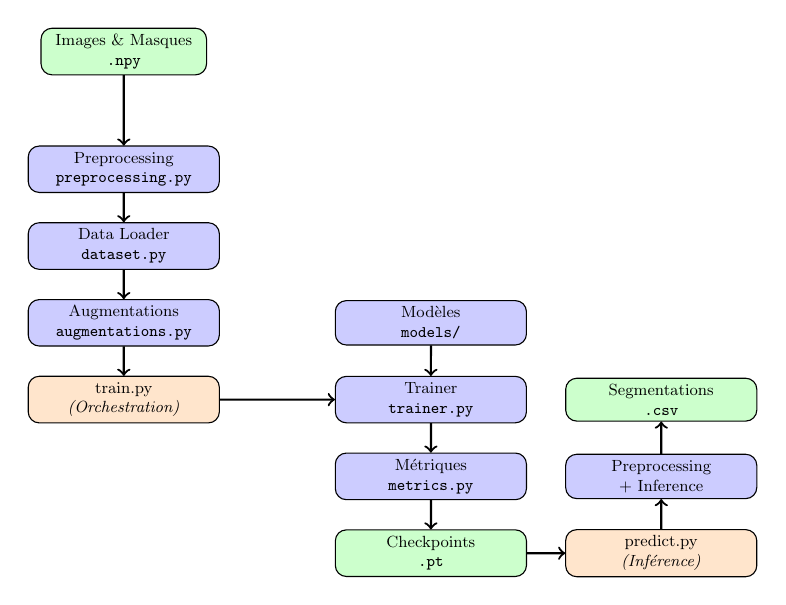
\begin{tikzpicture}[scale=0.65, transform shape, node distance=1.5cm, auto]
            % Define styles
            \tikzstyle{block} = [rectangle, draw, fill=blue!20, text width=3.5cm, text centered, rounded corners, minimum height=0.7cm, font=\small]
            \tikzstyle{data} = [rectangle, draw, fill=green!20, text width=3.5cm, text centered, rounded corners, minimum height=0.7cm, font=\small]
            \tikzstyle{entry} = [rectangle, draw, fill=orange!20, text width=3.5cm, text centered, rounded corners, minimum height=0.7cm, font=\small]
            \tikzstyle{arrow} = [thick, ->]

            % TRAINING PIPELINE (Left side)
            \node (input) [data, text width=3cm] {Images \& Masques\\ \texttt{.npy}};

            \node (preproc) [block, below of=input, yshift=-0.8cm] {Preprocessing\\ \texttt{preprocessing.py}};

            \node (dataloader) [block, below of=preproc] {Data Loader\\ \texttt{dataset.py}};

            \node (augment) [block, below of=dataloader] {Augmentations\\ \texttt{augmentations.py}};

            \node (train_entry) [entry, below of=augment] {train.py\\ \textit{(Orchestration)}};

            % Models (middle)
            \node (models) [block, right of=augment, xshift=4.5cm] {Modèles\\ \texttt{models/}};

            % Training Core
            \node (trainer) [block, right of=train_entry, xshift=4.5cm] {Trainer\\ \texttt{trainer.py}};

            % Evaluation
            \node (metrics) [block, below of=trainer] {Métriques\\ \texttt{metrics.py}};

            % Checkpoints
            \node (output) [data, below of=metrics] {Checkpoints\\ \texttt{.pt}};

            % INFERENCE PIPELINE (Right side)
            \node (predict_entry) [entry, right of=output, xshift=3cm] {predict.py\\ \textit{(Inférence)}};

            \node (inference) [block, above of=predict_entry] {Preprocessing\\ + Inference};

            \node (predictions) [data, above of=inference] {Segmentations\\ \texttt{.csv}};

            % Training pipeline arrows
            \draw [arrow] (input) -- (preproc);
            \draw [arrow] (preproc) -- (dataloader);
            \draw [arrow] (dataloader) -- (augment);
            \draw [arrow] (augment) -- (train_entry);
            \draw [arrow] (models) -- (trainer);
            \draw [arrow] (train_entry) -- (trainer);
            \draw [arrow] (trainer) -- (metrics);
            \draw [arrow] (metrics) -- (output);

            % Inference pipeline arrows
            \draw [arrow] (output) -- (predict_entry);
            \draw [arrow] (predict_entry) -- (inference);
            \draw [arrow] (inference) -- (predictions);

      \end{tikzpicture}
      \caption{Pipeline complet : entraînement (gauche) et inférence (droite)}
      \label{fig:architecture}
\end{figure}

Le schéma Figure~\ref{fig:architecture} illustre l'architecture modulaire du projet en deux phases distinctes:

\paragraph{Phase d'entraînement :}
Le pipeline orchestre l'ingestion des données brutes, leur prétraitement (normalisation, interpolation) et leur augmentation dynamique. Les \textit{DataLoaders} stratifiés alimentent la boucle d'apprentissage (\texttt{trainer.py}) qui gère la rétropropagation et l'évaluation continue des métriques. Un mécanisme d'\textit{Early Stopping} garantit la sauvegarde du modèle optimal.

\paragraph{Phase d'inférence :}
Le script \texttt{predict.py} exploite le meilleur checkpoint pour prédire les masques sur les données de test, en garantissant la cohérence des prétraitements avant l'export standardisé des résultats.

\subsubsection{Description des modules}

\begin{itemize}
      \item \textbf{preprocessing.py} : Normalisation min-max, interpolation des images manquantes,
            conversion des masques en format compatible PyTorch.

      \item \textbf{dataset.py} : Chargement des données, création des DataLoaders PyTorch,
            gestion des splits train/validation avec stratification par puits.

      \item \textbf{augmentations.py} : Implémentation des transformations géométriques
            (rotations, flips) et du bruit Gaussien appliqués dynamiquement en entraînement.

      \item \textbf{models/} : Définitions des architectures UNet, UNet avec encodeur pré-entraîné,
            et variantes avec attention mechanisms.

      \item \textbf{trainer.py} : Boucle d'entraînement complète incluant forward pass,
            calcul de loss, backward propagation, et sauvegarde du meilleur modèle via Early Stopping.

      \item \textbf{metrics.py} : Calcul de l'Intersection over Union (IoU) pour chaque classe
            et accumulation des métriques moyennes via la classe \texttt{MetricsTracker}.
            Assure le suivi continu des performances pendant l'entraînement et la validation.

      \item \textbf{train.py} : Point d'entrée principal orchestrant l'entraînement avec
            arguments en ligne de commande pour configurer le modèle, le dataset et les hyperparamètres.

      \item \textbf{predict.py} : Interface d'inférence permettant de générer des prédictions
            segmentation sur de nouvelles images.
\end{itemize}

\subsubsection{Modèle UNet Baseline}

Le modèle UNet \textit{baseline} constitue la référence de ce travail. Son architecture
suit la structure encodeur-décodeur classique, adaptée
à notre contexte d'images ultrasonores monocanal ($160 \times 160$ pixels).

\textbf{Architecture générale :}

\begin{itemize}
      \item \textbf{Encodeur} : 4 niveaux de convolution descendante avec max pooling
      \item \textbf{Goulot d'étranglement (Bottleneck)} : Bloc de convolution au niveau
            le plus profond
      \item \textbf{Décodeur} : 4 niveaux de déconvolution ascendante avec skip connections
      \item \textbf{Skip connections} : Concaténation des activations de l'encodeur aux
            niveaux correspondants du décodeur, préservant l'information spatiale
\end{itemize}

\textbf{Blocs constitutifs :}

Chaque niveau de l'encodeur et du décodeur utilise un \texttt{ConvBlock} composé de :
\[
      \boxed{\text{Conv2d}(k=3) \to \text{BatchNorm} \to \text{ReLU}} \quad \text{(appliqué 2 fois)}
\]

Cette structure double-convolution avec normalisation par batch stabilise l'apprentissage
et améliore la convergence. Le padding de 1 pixel préserve les dimensions spatiales au sein
de chaque bloc.

Ce modèle baseline sert de point de comparaison pour les architectures ultérieures
(avec Dropout, avec Focal Loss, avec transfer learning).

\subsubsection{Modifications ultérieures}

\paragraph{Ajout de Dropout :}

L'intégration de couches de \textit{Dropout} ($p=0.3$ après activation) a été évaluée comme stratégie de régularisation explicite pour prévenir le surapprentissage. Bien que théoriquement pertinente pour limiter la co-adaptation des neurones sur un dataset restreint, cette approche a empiriquement dégradé les performances par rapport au modèle de référence.
Cette contre-performance indique que la perturbation stochastique interne interfère avec l'apprentissage des structures spatiales cohérentes des images ultrasonores. Il apparaît que les régularisations existantes (augmentation de données, pondération des classes) assuraient déjà un contrôle efficace du surapprentissage, rendant l'ajout de bruit supplémentaire contre-productif pour la convergence du modèle.

\paragraph{Ajout de bruit Gaussien dans l'augmentation :}

Nous avons enrichi le pipeline d'augmentation par l'injection dynamique de bruit gaussien ($\sigma=0.02, p=30\%$) afin de simuler les artéfacts d'acquisition ultrasonores. L'objectif est d'accroître la robustesse du modèle face aux variations de signal sans altérer la sémantique structurelle des interfaces.

Les résultats montrent une efficacité contrastée selon l'architecture : alors que le modèle \textit{baseline} voit ses performances chuter face à ce bruit additionnel, les variantes pré-entraînées en bénéficient nettement. Ces dernières, grâce aux représentations robustes de leurs encodeurs (ResNet), exploitent efficacement ce bruit comme régularisateur, confirmant que la stratégie d'augmentation doit être calibrée en fonction de la capacité d'abstraction du réseau.

\paragraph{Exploration de fonctions de perte alternatives :}

Au-delà de la \textit{CrossEntropyLoss} standard, nous avons évalué l'impact de critères d'optimisation spécifiques à la segmentation déséquilibrée :
\begin{itemize}
      \item \textbf{Focal Loss} ($\gamma=2.0$) : Conçue pour focaliser l'apprentissage sur les exemples difficiles ("hard negatives") afin de compenser le déséquilibre de classes (TIE $\approx$ 6\%, Casing $\approx$ 9\%).
      \item \textbf{Dice Loss} : Vise l'optimisation directe de la métrique IoU en maximisant le recouvrement spatial, favorisant ainsi la cohérence géométrique des prédictions.
      \item \textbf{Combined Loss} ($\mathcal{L}_{CE} + 0.5 \cdot \mathcal{L}_{Dice}$) : Approche hybride combinant la robustesse probabiliste de l'entropie croisée et la précision surfacique de la Dice Loss.
\end{itemize}

Les résultats indiquent que la \textit{Focal Loss} n'offre pas de gain significatif face à une \textit{Weighted CrossEntropy}, la pondération des classes suffisant apparemment à gérer le déséquilibre. En revanche, l'usage de la \textit{Dice Loss} s'est avéré déterminant pour les performances finales des modèles avancés.
\paragraph{Intégration d'Attention Gates :}

Afin d'optimiser le transfert d'information via les \textit{skip connections}, nous avons intégré des modules d'\textit{Attention Gates} (AG). Contrairement à la concaténation standard qui fusionne toutes les caractéristiques spatiales sans distinction, les AG filtrent le signal de l'encodeur ($\mathbf{x}$) en se basant sur le contexte sémantique fourni par le décodeur ($\mathbf{g}$). Le mécanisme $\hat{\mathbf{x}} = \sigma(\psi(\mathbf{x}, \mathbf{g})) \odot \mathbf{x}$ génère une carte de saillance qui pondère les activations, amplifiant les zones pertinentes tout en atténuant le bruit de fond.

Cette modification architecturale s'est révélée bénéfique, surpassant les performances du modèle de base. En agissant comme un mécanisme de sélection adaptative, l'attention permet au réseau de focaliser ses ressources sur les régions d'intérêt (interfaces fines), améliorant la précision de délimitation conformément à l'état de l'art en segmentation d'images.

\paragraph{Utilisation d'encodeurs pré-entraînés (Transfer Learning) :}

Pour pallier la limitation du volume de données, nous avons substitué l'encodeur standard par des architectures \textit{ResNet} pré-entraînées sur ImageNet. Cette approche de \textit{transfer learning} exploite la hiérarchie de caractéristiques visuelles déjà acquises : les couches superficielles détectent les primitives universelles (textures, contours) tandis que les couches profondes encodent des abstractions sémantiques robustes. Outre l'accélération de la convergence, cette initialisation réduit drastiquement le risque de surapprentissage inhérent aux petits datasets.

La stratégie d'implémentation repose sur un protocole en deux phases :
\begin{enumerate}
      \item \textbf{Initialisation du décodeur} : L'encodeur est gelé (\textit{frozen}) pour forcer l'adaptation exclusive du décodeur aux représentations fixes, prévenant la dégradation des poids pré-appris par des gradients instables (LR : $1\cdot10^{-3}$).
      \item \textbf{Raffinement global} : libération de l'encodeur pour un \textit{fine-tuning} complet à très faible taux d'apprentissage ($1\cdot10^{-4}$), permettant une adaptation fine aux spécificités de l'imagerie ultrasonore sans oubli catastrophique.
\end{enumerate}

Par souci de temps, nous n'avons testé que ResNet34, qui semblait être le bon compromis entre capacité et temps.

\textbf{*Disclaimer}: je me suis rendu compte que pour la moitié des réseaux préentraînés, on n'a pas utilisé la phase 1 de l'entraînement !! (problème d'écriture de ligne de commande).
On verra que ça n'a pas beaucoup d'incidence néanmoins.